\documentclass[a4paper, oneside]{memoir}

\usepackage[rgb]{xcolor}
\usepackage{tikz}
\usetikzlibrary{backgrounds}
\usepackage{pgfplots}
\usepackage{bookmark}
\usepackage{booktabs}
\usepackage{array}
\usepackage{hyperref}
\usepackage{enumitem}
\usepackage{graphicx}
\usepackage{wrapfig}
\usepackage{listings}
\usepackage{amsmath}
\usepackage{bytefield}
\usepackage{siunitx}
\usepackage{natbib}

\setlength{\parskip}{0.5\baselineskip}

\setlength\cftchapterindent{\cftsectionindent}
\setlength\cftbeforechapterskip{0pt}
\renewcommand\cftchapterpagefont{\normalfont}

\renewcommand{\cftchapterleader}{\cftdotfill{\cftdotsep}}

\setlrmarginsandblock{1.25in}{1.25in}{*} 
\setulmarginsandblock{1.25in}{1.25in}{*} 
\checkandfixthelayout%

\renewcommand{\thesection}{\arabic{section}}
\renewcommand{\thefigure}{\arabic{figure}}
\renewcommand{\thetable}{\arabic{table}}

\lstset{language=C++,
                basicstyle=\ttfamily,
                keywordstyle=\color{blue}\ttfamily,
                stringstyle=\color{red}\ttfamily,
                commentstyle=\color{lightgreen}\ttfamily,
                morecomment=[l][\color{magenta}]{\#}
}

\newcommand*{\semester}[2]{Semester #1 -- #2} %chktex 8
\newcommand*{\student}[3]{&\text{#1} &\text{#2} &&\text{#3}} %chktex 8
\newcommand*{\titleAM}[3]%
{\begingroup
  \centering
  {\Huge #1:\\#2\par}\vspace{\baselineskip} % Fixed newline error
  {\small\scshape RMIT University}\par
  {\small\scshape #3}\par\vspace{0.5em}
  \endgroup}

\renewcommand{\tocheadstart}{}
\renewcommand{\aftertoctitle}{}
\renewcommand{\printtoctitle}[1]{}
\setcounter{secnumdepth}{3}
\setcounter{tocdepth}{3}

\makeatletter
\DeclareRobustCommand{\cskippedwords}[2][2ex]{%
  \setlength{\units@wide}{\bf@bitwidth * \bits@wide}%
  \setlength{\units@high}{1pt * \ratio{\units@wide}{6.0pt}}%
  \setlength{\units@tall}{#1 + \units@high}%
  \edef\num@wide{\strip@pt\units@wide}%
  \edef\num@tall{\strip@pt\units@tall}%
  \edef\num@high{\strip@pt\units@high}%
  \begin{picture}(\num@wide,\num@tall)%
  \begin{tikzpicture}[overlay]
  \draw[fill=#2,fill opacity=0.2] 
    (0,-\bf@bitheight) -- (0,0) -- (0,\units@high) -- (\units@wide,0) -- +(0,-\bf@bitheight) -- cycle;
  \draw[fill=#2,fill opacity=0.2]
    (0,\units@high+#1+\bf@bitheight) -- ++(\units@wide,0) -- ++(0,-\bf@bitheight-\units@high) -- (0,\units@high+#1) -- cycle;
  \end{tikzpicture}%
  \end{picture}%
  \ifcounting@words
    \inc@bytefield@height{\unitlength * \real{\num@tall}}%
    \global\counting@wordsfalse
  \fi}
\makeatother

\definecolor{bittersweet}{rgb}{1.0, 0.44, 0.37}
\definecolor{aquamarine}{rgb}{0.5, 1.0, 0.83}
\definecolor{lavender}{rgb}{0.9, 0.9, 0.98}
\definecolor{whitesmoke}{rgb}{0.96, 0.96, 0.96}
\definecolor{lightgreen}{RGB}{102,153,0}    %#669900

\lstset{language=C++,
        basicstyle=\ttfamily,
        keywordstyle=\color{blue}\ttfamily,
        stringstyle=\color{red}\ttfamily,
        commentstyle=\color{lightgreen}\ttfamily,
        morecomment=[l][\color{magenta}]{\#},
        backgroundcolor=\color{whitesmoke}
}

\renewcommand{\bibname}{References}
\newlist{questions}{enumerate}{2}
\setlist[questions,1]{label=RQ\arabic*.,ref=RQ\arabic*}
\setlist[questions,2]{label= (\alph*),ref=\thequestionsi(\alph*)}

\begin{document}
\titleAM{Programming Autonomous Robots}{Robotics Project}{\semester{1}{2024}}
  \begin{align*}
    &\text{Name} &\text{Student No.} &&\text{Contribution}\\
    \student{Matthew Ricci}{s3785111}{33\%}\\
    \student{Noah Solman}{s3285661}{33\%}\\
    \student{Bailey Vogt}{s3906263}{33\%}
  \end{align*}
  \addcontentsline{toc}{part}{Contents}
  \tableofcontents*
  \clearpage
  \renewcommand{\abstractname}{Summary}

  \markboth{}{}
  \section{Introduction}


    \setlength{\intextsep}{0pt}
    \begin{wrapfigure}{r}{\textwidth/2}
        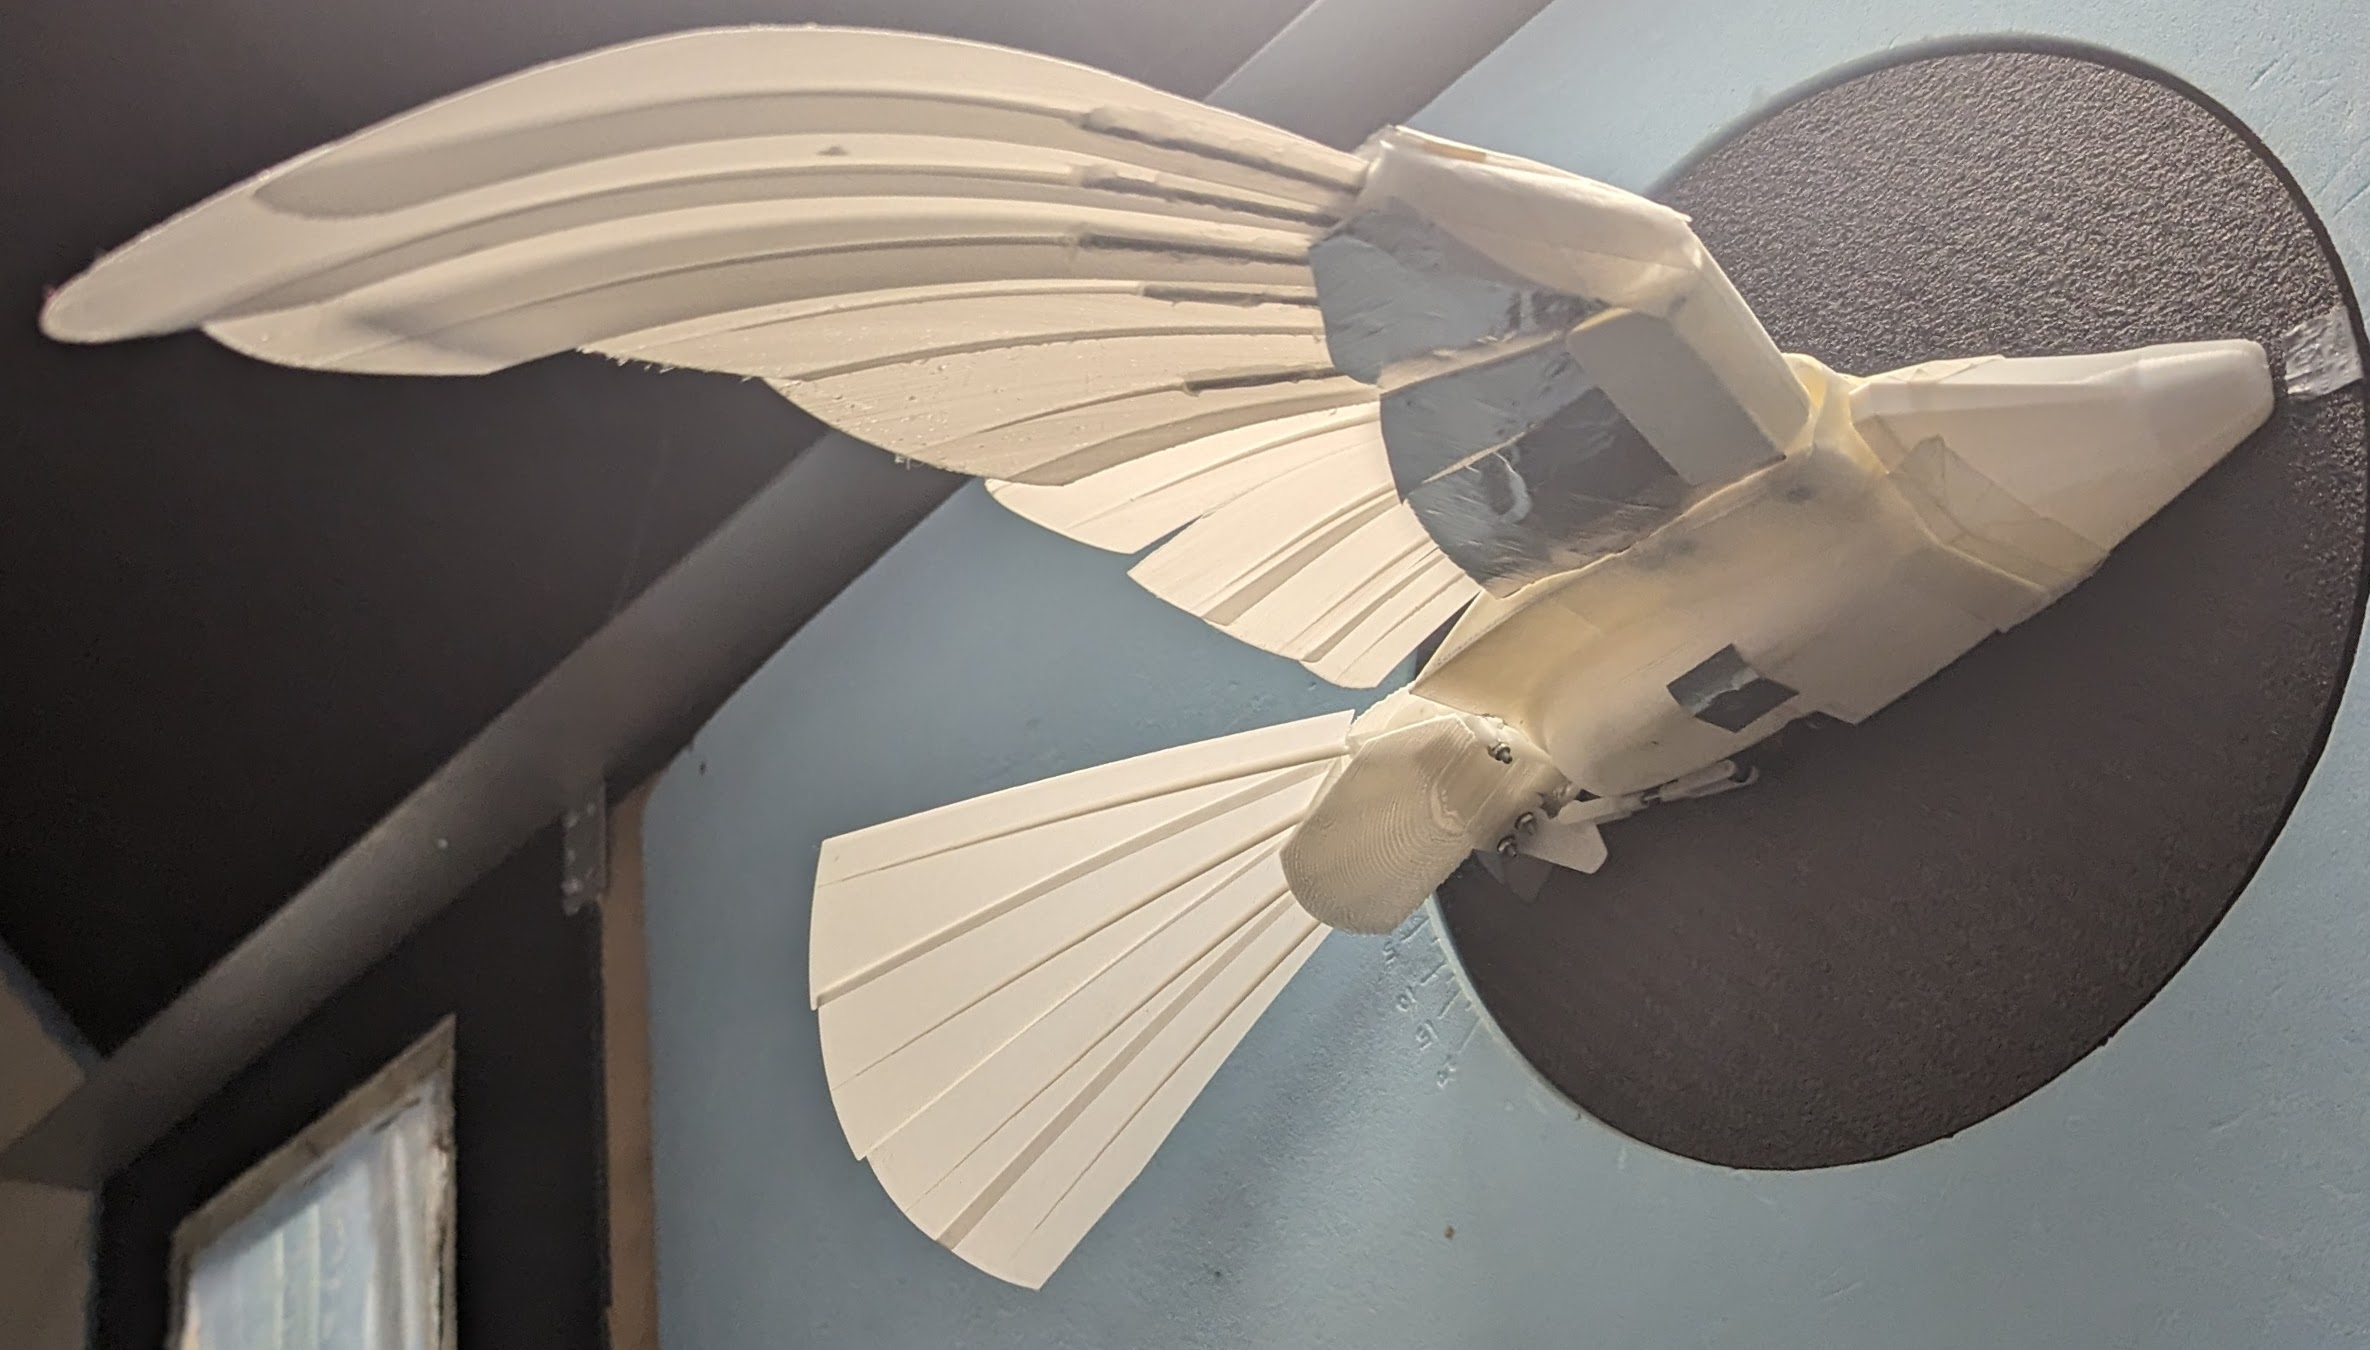
\includegraphics[width=\textwidth/2]{./Resources/Kestrel.jpg}
        \caption{\label{fig:figure 1} Kestrel Bird System}
    \end{wrapfigure}
    Mapping and surveying, environmental monitoring, delivery, search and
    rescue are some of the current applications of Unmanned Arial Vehicles
    (UAVs). Improving their ability to adjust to changes in wind conditions
    is a topic of much research [1] especially as work continues to
    allow UAVs to carry out increasingly complicated tasks autonomously
    like CSIRO’s Hovermap an arial 3D mapping platform [2].
    \vspace{\baselineskip}
    In Australia the height limit to operate a UAV is 120m above ground
    level [3]. At these heights wind turbulence and gust conditions greatly
    impact the performance of UAVs, by changing its trajectory and expected
    current state potentially leading to drone damage. As a response to
    this, researchers have turned to nature as inspiration. Basing UAV
    design on birds has advantages over classical UAV designs (like
    multi-rotor or fixed wing drones) including increased aerodynamic
    efficiency, high manoeuvrability and stability in high-gust conditions
    [4].
    \vspace{\baselineskip}
    In this project we build on existing work to develop stable flight
    controllers for a novel platform the Kestrel robotic replica half-wing
    based on the Nankeen Kestrel with three degrees of freedom (wing
    extension, tail spread and tail pitch) [5]
    (Figure 1).
    As a novel design
    the wing cannot be controlled with existing software, prior work on the
    Kestrel half-wing focussed on utilising Deep Reinforcement Learning
    (DRL) to develop a flight stability controller. DRL has been shown
    to have superior response time, reduced error and ability to reject
    external disturbances. Additionally, development of a DRL controller
    does not require domain specific knowledge in controller tuning [6].
    \vspace{\baselineskip}
    We will investigate the use of a classical controllers on the novel
    Kestrel platform to directly compare it to the DRL controller.
    We aim develop a Proportional Integral Derivative (PID) controller
    for flight stability already shown to be effective in stabilising UAVs
    [7].
    \vspace{\baselineskip}

\section{Related Work}
    PID control systems have been extensively explored in UAV
    stabilisation. According to a 2023 survey, Lopez-Sanchez et al.
    conducted an exhaustive literature review and realized that the most
    common control technique for quadrotor UAVs is PID control [7]. With
    adaptive PID control being the most stable under unstable conditions,
    providing robustness against parameter uncertainty. An adaptive PID
    changes the gains of the controller during flight based on performance
    evaluation loop built into the controller. As all our testing will be
    conducted in laminar flow, an adaptive PID will not be implemented and a
    classical PID will be developed to reduce complexity of implementation.
    \vspace{\baselineskip}
    Tuning a PID using trial-and-error is a manual, tedious process often
    requiring expert domain knowledge [6]. To address this, researchers are
    applying machine learning to the problem of finding high-performing gains
    for PID controllers. Support Vector Regression (SVR) is increasingly being
    used for PID controllers to facilitate the tuning process. Studies have
    shown that SVR-based controllers display enhanced stability and accuracy
    in variety of applications [8].
    \vspace{\baselineskip}
    In terms of applications in bio-inspired wings, Wenfu et al. in a 2021
    experiment showed the effectiveness of implementing a PID in a robotic
    bird. They describe that as their bird gets more complex, increasingly
    complex methods of control will be required. 
    \vspace{\baselineskip}
    As Okasha et al. discussed in their 2022 paper. Model Predictive Control
    (MPC) is a powerful controller that is more robust and stable compared
    to PID, though it is computationally expensive [10]. Another advantage
    over PID is that it bypasses the tuning phase.
    \vspace{\baselineskip}
    The existing literature on PID, SVR tuning and MPC in the UAV space
    provided valuable insights for our project. By learning from these
    approaches, we can utilise a variety of control methods in a novel
    platform the Kestrel bio-inspired wing.

\section{Methodology}
    \subsection{System architecture}

    \subsection{Software architecture}

    \subsection{Experiment details}
    \setlength{\intextsep}{0pt}
    \begin{wrapfigure}{r}{\textwidth/2}
        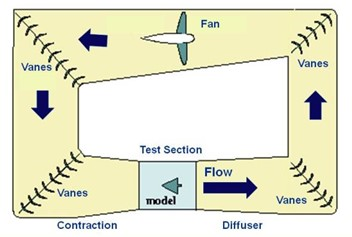
\includegraphics[width=\textwidth/2]{./Resources/Fig2_wind_tunnel_design.jpg}
        \caption{\label{fig:figure 2} Closed Return Wind Tunnel [10]}
    \end{wrapfigure}
    \quad\textbf{Wind tunnel}\\
    The Kestrel will be mounted in the blue wind tunnel at the RMIT
    Bundoora Campus. It is a closed return wind tunnel [11]. The
    wind tunnel is built across two floors with wind generated by a fan on
    the first floor sent to the second floor where the testing area is.
    This design ensures steady delivery of laminar flow, wind flow without
    disturbances. Figure 2 from displays this generic design. The vanes on
    each corner of the tunnel ensure that the flow is laminar. 
    \vspace{\baselineskip}
    A pressure probe embedded in the test area allows us to assess the
    pressure in the wind tunnel. Knowing the target speed and the ambient
    temperature and air pressure of the wind tunnel allows us to calculate
    a target pressure which is what we aim for when testing. All our testing
    occurred at approximately 0.0155 kPa or 5 m/s, the target pressure would
    fluctuate throughout the day as ambient temperature and pressures
    changed. As such we regularly calculated the target pressure to ensure
    consistent speeds.
    \vspace{\baselineskip}

    \setlength{\intextsep}{0pt}
    \begin{wrapfigure}{r}{\textwidth/2}
        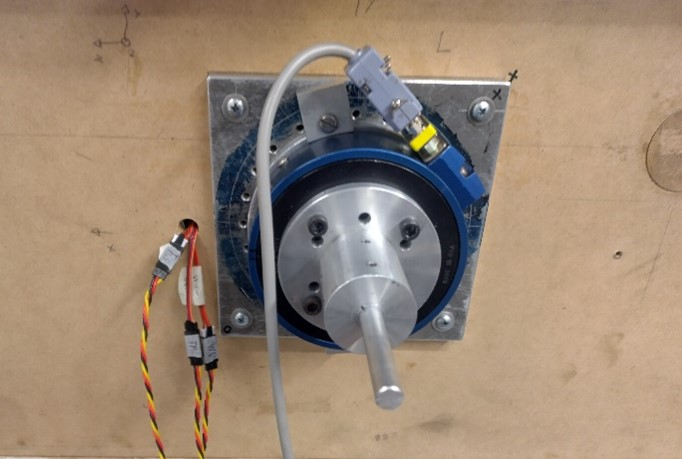
\includegraphics[width=\textwidth/2]{./Resources/Fig3_load_cell.jpg}
        \caption{\label{fig:figure 3} 30N Load Cell}
    \end{wrapfigure}
    \quad\textbf{Load cell}\\
    The Kestrel is mounted directly onto a 30 N load cell (Figure 3). The
    output from the load cell describes the major forces occurring on the
    Kestrel. After processing through the data acquisition box, we are given
    a list of 6 values: the force in N at X, Y and Z. We are also given
    moments in X, Y and Z, which is expressed in Nm. The primary force used
    in training and testing was the force at Y or the lift.
    \vspace{\baselineskip}
    Before each test the load cell must be calibrated to ensure we return
    accurate results. In our design we take 1000 results from the load cell
    and store the average for each measure in a file. This average is then
    subtracted from each test measurement to zero the load cell. We recognised
    some drift in the load cell and therefor we calibrated the load cell regularly.
    \vspace{\baselineskip}

    \quad\textbf{Data output}\\
    After a test everything that happens at each timestep this includes all the
    forces in N and moments in Nm, the new set position of each servo as decided by
    the controller and the error lift. For all tests the lift of the bird was
    targeted to be 0.42 N.
    This data will be sufficient to capture our primary outcomes:

        • Time taken to stabilise the bird

        • Quality of transition to stability

        • Quality of stability (error is as close to zero as possible throughout flight)
    In addition to assessing the robustness of our controllers the output will
    allow us to compare to the pre-trained DRL model.
    The following is the experimental workflow that was carried out to conduct each major test.

        1. Load cell calibration, to zero the load cell

        2. Dynamic pressure assessment, to ensure consistent speeds

        3. Set wind speed, based on dynamic pressure assessment

        4. Run test of interest PID / MPC / SVR tuner

        5. Data collection



\section{Results}
\section{Evaluation}
\section{Discussion}
\section{Conclusion}
\section{References}

        
  \bibliographystyle{ieeetr}
  \bibliography{robotics_project}


  %\renewcommand{\thechapter}{\Alph{chapter}}
\renewcommand{\thefigure}{\Alph{chapter}.\arabic{figure}}
\renewcommand{\chaptername}{Appendix}
\addcontentsline{toc}{part}{Appendix}

\clearpage
\chapter{}\label{apdx:A}
\setlrmarginsandblock{0.5cm}{0.5cm}{*}
\checkandfixthelayout
\vfill{}
\begin{figure}[h]
  \begin{center}
    \includegraphics[width=\textwidth]{./img/}
  \end{center}
\end{figure}
\vfill{}

\end{document}
